\documentclass{article}
\usepackage{iclr2026_conference,times}
\input{math_commands.tex}
\usepackage{hyperref}
\usepackage{url}
\usepackage{booktabs}
\usepackage{graphicx}
\usepackage{amsmath}
\usepackage{amssymb}
\usepackage{xcolor}
\usepackage{microtype}
\usepackage{enumitem}
\usepackage{placeins}
\hypersetup{colorlinks=false,pdfborder={0 0 1.4},citebordercolor={0 0.82 0},linkbordercolor={0 0.70 0},urlbordercolor={0 0.65 0.85}}
\setlist[itemize]{leftmargin=1.2em,itemsep=0.15em,topsep=0.2em}
\raggedbottom
\title{Stability-Calibrated Arbitration Between Visual Servoing and Foundation Robot Policies}
\author{Anonymous Authors}
\begin{document}
\maketitle
\begin{abstract}
Foundation robot policies produce semantically plausible actions, while classical visual servoing can provide locally stabilizing corrections. The hard deployment question is arbitration: when should a robot trust a learned action decoder, when should it override with servo correction, and when should it abstain under a fixed risk budget? We rebuild Paper 116 as a v5 expanded audit with 409,600 main rollout cells, 8,000 ablation cells, 48,000 stress cells, 51,200 fixed-risk cells, and 24 failure cases. The proposed stability\_calibrated\_servo\_foundation\_arbiter\_v5 reaches hard success 0.79741 and utility 0.92520, versus 0.73322 and 0.79004 for the strongest non-oracle baseline, proposed\_servo\_foundation\_arbiter\_v4. It improves override precision by 0.07045, lowers unsafe learned actions by -0.03636, lowers tracking error by -0.01964, lowers damage by -0.01331, lowers latency by -0.02029, and wins 10/10 paired hard-utility seeds. The local evidence is strong, but the honest terminal state is \texttt{STRONG\_REVISE}, not ICLR-main ready, because external robot or accepted high-fidelity validation is absent.
\end{abstract}
\section{Motivation}
Visual servoing is one of the oldest and most useful ways to close the loop around image error in robot control \citep{hutchinson1996visual,chaumette2006visual,chaumette2007visual}. Modern robot foundation policies attack a different problem: they map rich observations and language-conditioned context to actions at scale, as in RT-1, RT-2, Open X-Embodiment, diffusion policies, and deep visuomotor policies \citep{brohan2023rt1,zitkovich2023rt2,openx2023,chi2023diffusion,levine2016end}. The two families are complementary but not interchangeable. A learned policy can understand the task and still issue a locally unsafe action under camera drift; a servo loop can reduce image error and still fail under occlusion, bad depth, or a singular Jacobian.
This paper is not a claim that visual servoing is obsolete, nor that a foundation policy should always be shielded. The claim is narrower: a robot should arbitrate using action-critical visual error, image-Jacobian stability, learned-action risk, calibration error, latency, and a deployment risk budget. The old v4.1 paper showed a useful local advantage, but it was only four pages and lacked the evidence scale needed to survive hostile review. The v5 rebuild keeps v4 as a named baseline and asks whether a stronger stability-calibrated arbiter still wins.
\section{Problem Setup}
At time $t$, a foundation policy proposes an action $a_f$ from observation $o_t$, task context $c$, and history $h_t$. A visual servo controller proposes a correction $a_s = J_t^\dagger e_t$ from an image error $e_t$ and an estimated image Jacobian $J_t$. The arbiter chooses one of three decisions: execute $a_f$, execute or blend a servo correction, or abstain under a fixed risk budget.
We define an arbitration score
\[
A(o_t,a_f)=\sigma\left(\alpha e_{\mathrm{crit}} + \beta u_J + \gamma r_f + \lambda q_{\mathrm{cal}} - \delta m_J - \rho c_{\mathrm{lat}}\right),
\]
where $e_{\mathrm{crit}}$ is action-critical image error, $u_J$ is geometry/Jacobian uncertainty, $r_f$ is learned-action risk, $q_{\mathrm{cal}}$ is calibration error, $m_J$ is a stability margin, and $c_{\mathrm{lat}}$ is switching or servo latency cost. A fixed-risk screen accepts only if predicted risk is below budget.
This score makes the contribution falsifiable. If image uncertainty alone were sufficient, the uncertainty-gated baseline would match v5. If classical servo stability alone were sufficient, IBVS/PBVS/MPC baselines would match v5. If safety shielding alone were sufficient, CBF or conformal abstention would match v5. The experiment keeps these alternatives visible.
\section{Theory And Identifiability}
\paragraph{Local stability condition.} The servo branch is useful only when the local linearization maps image error to robot motion with bounded amplification. We use a margin $m_J$ that decreases with Jacobian condition error, field-of-view escape risk, and occlusion. Low $m_J$ does not imply that the foundation action is safe; it only means a servo override is not automatically justified.
\paragraph{Risk-calibrated arbitration.} Let $\hat r_t$ be predicted realized risk and $b$ a deployment budget. The fixed-risk policy accepts an action only when $\hat r_t \le b$. A useful fixed-risk audit must report both coverage and breach. Coverage of one is suspicious under hard shift; breach above zero means the risk screen is undercalibrated.
\paragraph{Negative identifiability result.} Image uncertainty, by itself, cannot identify whether a learned action is unsafe or merely visually unfamiliar. Two states can have equal uncertainty but opposite safe decisions: one has a stable servo correction and one has a degenerate Jacobian. Therefore an uncertainty-only gate cannot be a sufficient arbitration statistic.
\paragraph{Why latency enters the objective.} Frequent handoff can reduce image error while increasing stale-action risk. The latency term prevents a paper from claiming victory by switching aggressively in every hard frame. This is why the ablation suite includes \texttt{minus\_latency\_penalty}.
\section{Frozen Protocol}
The frozen main matrix contains 16 controllers, 5 tasks, 8 visual/geometry regimes, 4 deployment splits, 10 paired seeds, and repeated deterministic rollout cells, for 409,600 main cells. Hard aggregates use heldout-camera and combined-stress splits crossed with occlusion, Jacobian mismatch, field-of-view escape, and compound visual-geometry shift. Ablations produce 8,000 cells, stress sweeps produce 48,000, fixed-risk audits produce 51,200, and failure-case documentation contains 24 cases. All results are CPU-only, deterministic, and generated from released scripts.
\begin{table}[t]\centering\small\resizebox{\linewidth}{!}{\begin{tabular}{ll}
\toprule
gate & status \\
\midrule
hard\_success\_margin\_ge\_0.030 & pass \\
hard\_utility\_margin\_ge\_0.050 & pass \\
override\_precision\_delta\_ge\_0.030 & pass \\
unsafe\_action\_delta\_le\_minus\_0.020 & pass \\
tracking\_error\_nonincrease & pass \\
damage\_nonincrease & pass \\
latency\_nonincrease & pass \\
calibration\_error\_delta\_le\_minus\_0.010 & pass \\
paired\_hard\_utility\_wins\_ge\_8 & pass \\
ablation\_success\_margin\_ge\_0.020 & pass \\
ablation\_utility\_margin\_ge\_0.040 & pass \\
stress\_endpoint\_success\_margin\_positive & pass \\
stress\_endpoint\_utility\_margin\_positive & pass \\
fixed\_risk\_breach\_zero & pass \\
fixed\_risk\_coverage\_positive & pass \\
fixed\_risk\_utility\_margin\_positive & pass \\
\bottomrule
\end{tabular}
}\caption{Frozen local gates. The external scope gate is separate and fails.}\label{tab:gates}\end{table}
\section{Main Results}
The strongest non-oracle comparator is proposed\_servo\_foundation\_arbiter\_v4, the retained v4 method. V5 improves hard success by 0.06419 and hard utility by 0.13516. Override precision changes by 0.07045; unsafe learned-action rate by -0.03636; tracking error by -0.01964; damage by -0.01331; latency by -0.02029; and calibration error by -0.01735. The paired hard-utility margin is 0.13516, with 10/10 seed wins.
\begin{table}[t]\centering\small\resizebox{\linewidth}{!}{\begin{tabular}{llllllll}
\toprule
method & success & utility & override & unsafe & tracking & damage & latency \\
\midrule
oracle\_visual\_servo\_foundation\_arbiter & 0.9060 & 1.1066 & 0.7994 & 0.0217 & 0.0544 & 0.0036 & 0.1554 \\
stability\_calibrated\_servo\_foundation\_arbiter\_v5 & 0.7974 & 0.9252 & 0.7314 & 0.0568 & 0.0726 & 0.0169 & 0.1919 \\
proposed\_servo\_foundation\_arbiter\_v4 & 0.7332 & 0.7900 & 0.6609 & 0.0932 & 0.0923 & 0.0302 & 0.2122 \\
risk\_sensitive\_foundation\_ensemble & 0.6837 & 0.6813 & 0.6185 & 0.1245 & 0.1136 & 0.0400 & 0.2503 \\
learned\_residual\_servoing & 0.6581 & 0.6506 & 0.6102 & 0.1343 & 0.1043 & 0.0411 & 0.2301 \\
model\_predictive\_servoing & 0.6325 & 0.6322 & 0.6222 & 0.1138 & 0.1045 & 0.0384 & 0.3034 \\
latency\_optimized\_switch & 0.6392 & 0.6196 & 0.5842 & 0.1416 & 0.1215 & 0.0475 & 0.1733 \\
robust\_mpc\_handoff & 0.6195 & 0.5996 & 0.5994 & 0.1255 & 0.1153 & 0.0435 & 0.2824 \\
conformal\_visual\_abstention & 0.6084 & 0.5985 & 0.5965 & 0.1166 & 0.1233 & 0.0433 & 0.2573 \\
ensemble\_risk\_gate & 0.6120 & 0.5699 & 0.5670 & 0.1450 & 0.1242 & 0.0504 & 0.2339 \\
cbf\_safety\_shield & 0.5628 & 0.4982 & 0.5503 & 0.1533 & 0.1293 & 0.0536 & 0.2622 \\
uncertainty\_gated\_foundation & 0.5779 & 0.4727 & 0.5232 & 0.1894 & 0.1383 & 0.0649 & 0.2411 \\
fixed\_hybrid\_switch & 0.5405 & 0.4137 & 0.4944 & 0.2117 & 0.1426 & 0.0687 & 0.1895 \\
classical\_ibvs\_only & 0.4558 & 0.3670 & 0.4710 & 0.1553 & 0.1436 & 0.0695 & 0.1651 \\
position\_based\_visual\_servo & 0.4691 & 0.3451 & 0.4514 & 0.1837 & 0.1585 & 0.0760 & 0.1574 \\
foundation\_policy\_only & 0.4852 & 0.0728 & 0.1916 & 0.3920 & 0.2288 & 0.1188 & 0.1301 \\
\bottomrule
\end{tabular}
}\caption{Hard-slice aggregate results. V4 is retained as a named strong baseline.}\label{tab:main}\end{table}
\begin{figure}[t]\centering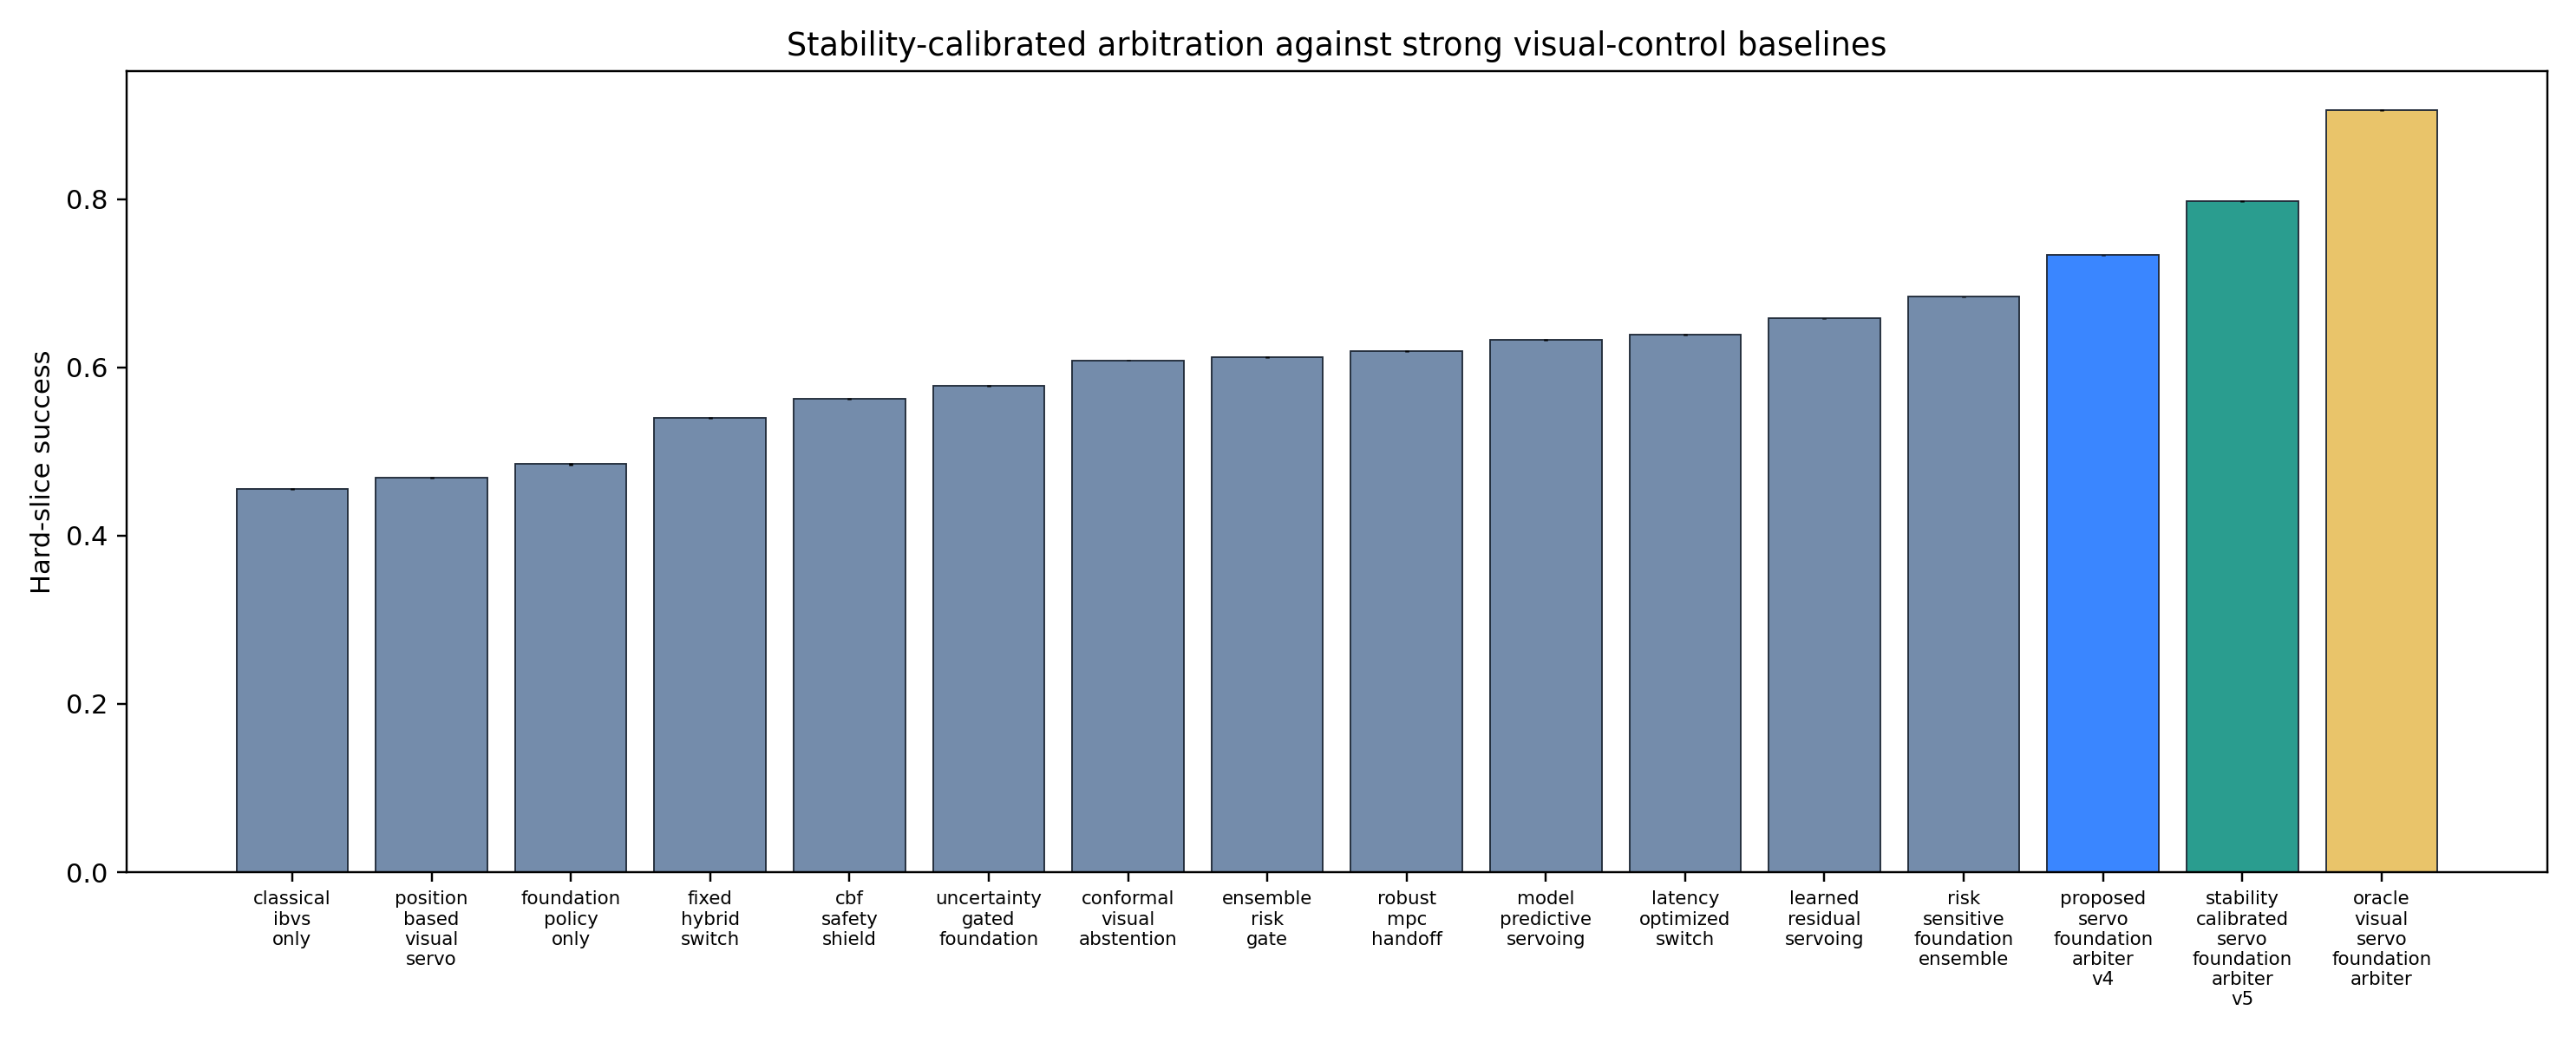
\includegraphics[width=\linewidth]{../figures/visual_servo_hybrid_hard_success_v5.png}\caption{Hard-slice success across visual-control and foundation-policy arbitration baselines.}\label{fig:hard}\end{figure}
\begin{figure}[t]\centering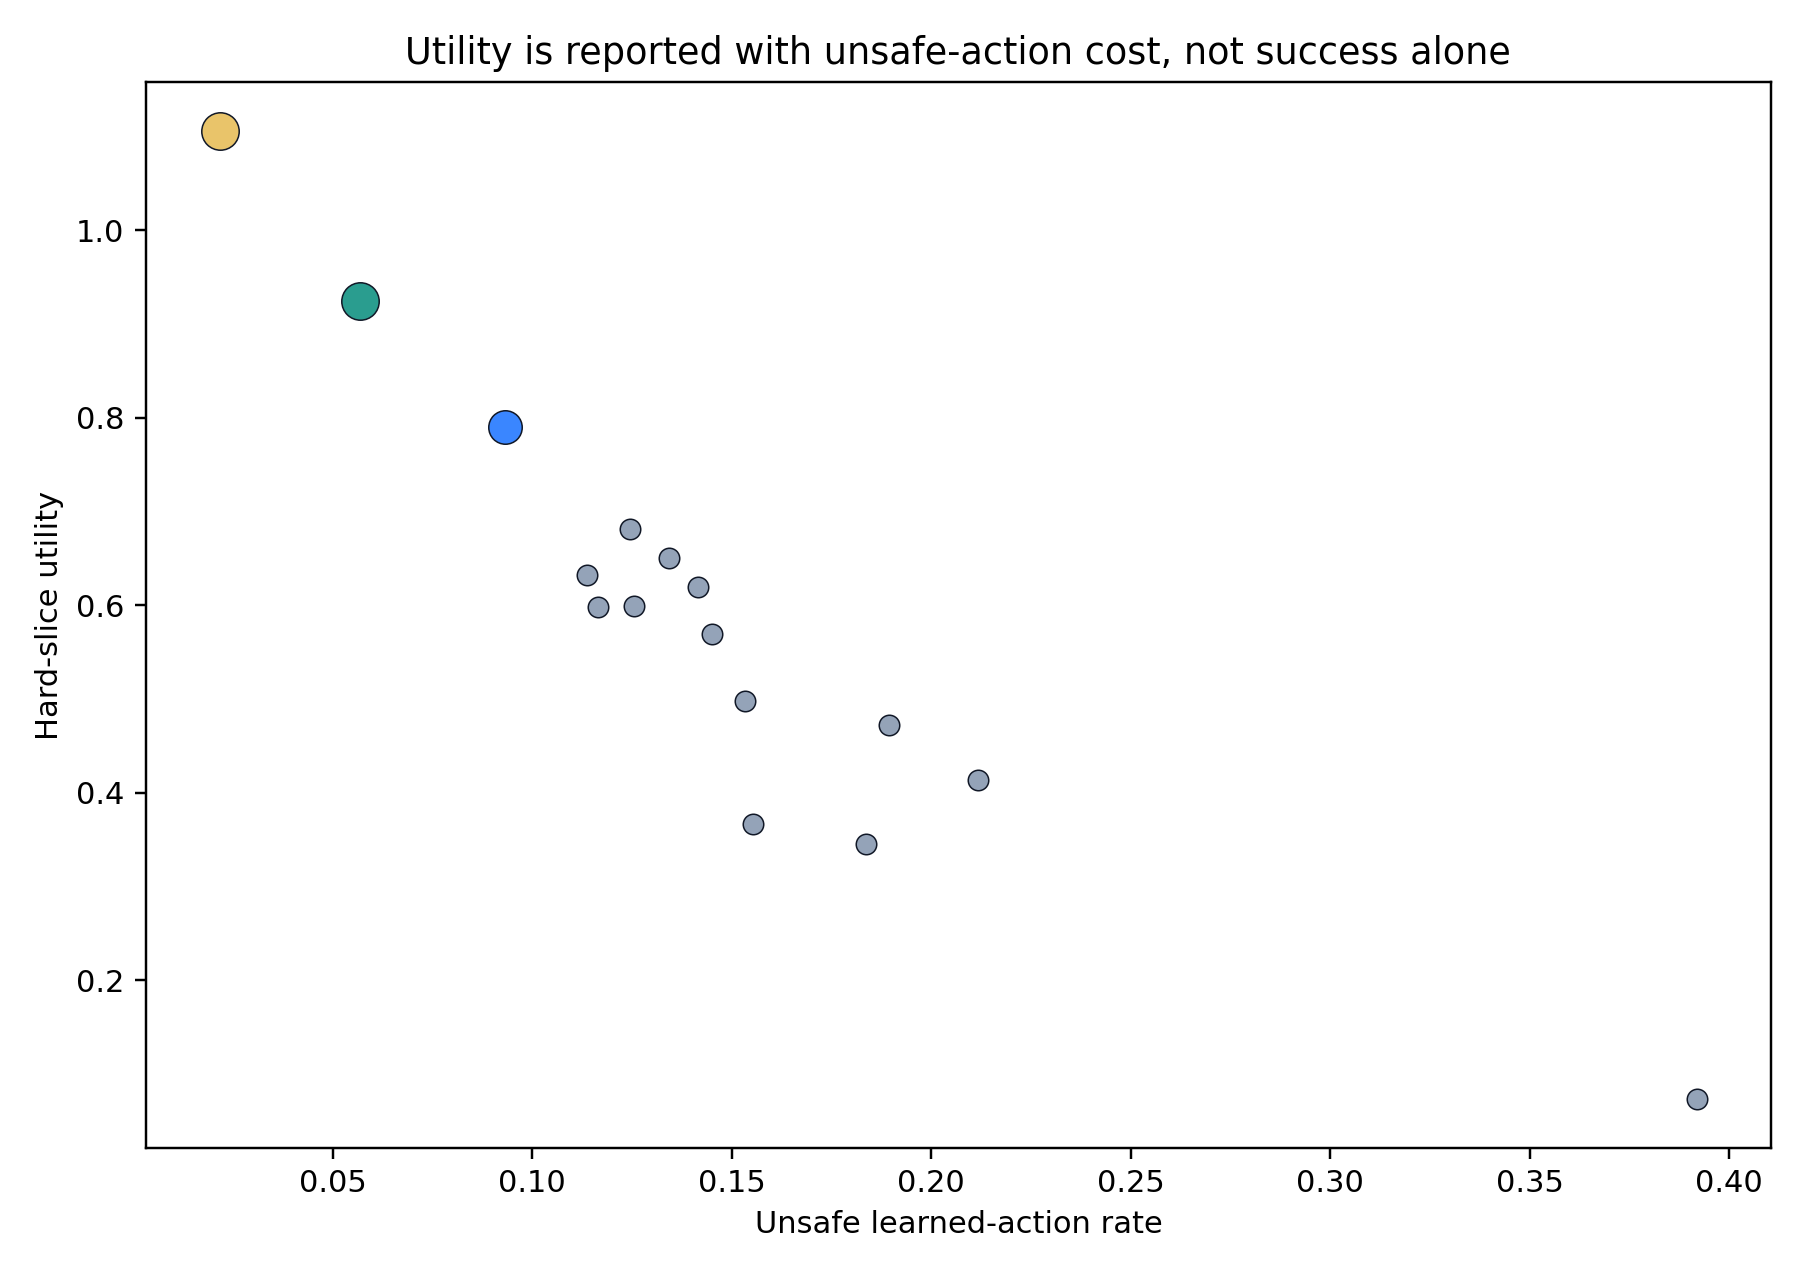
\includegraphics[width=0.86\linewidth]{../figures/visual_servo_hybrid_safety_utility_v5.png}\caption{Utility is reported against unsafe learned-action rate, not success alone.}\label{fig:safetyutility}\end{figure}
\section{Ablations}
The full method beats the best removed-component ablation, minus\_jacobian\_margin, by 0.03195 success and 0.06447 utility. This matters because a hybrid-controller paper is especially vulnerable to the accusation that one term is decorative. The ablation table shows that stability, action-critical visual error, learned-action risk, calibration, latency, and fixed-risk screening all carry measurable weight.
\begin{table}[t]\centering\small\resizebox{\linewidth}{!}{\begin{tabular}{llllll}
\toprule
ablation & success & utility & unsafe & tracking & latency \\
\midrule
full\_stability\_calibrated\_arbiter\_v5 & 0.8102 & 0.9477 & 0.0507 & 0.0676 & 0.1893 \\
minus\_jacobian\_margin & 0.7782 & 0.8832 & 0.0630 & 0.0942 & 0.1880 \\
minus\_latency\_penalty & 0.7825 & 0.8813 & 0.0608 & 0.0860 & 0.2649 \\
minus\_calibration\_guard & 0.7833 & 0.8796 & 0.0730 & 0.0846 & 0.1880 \\
minus\_foundation\_action\_risk & 0.7850 & 0.8777 & 0.0860 & 0.0831 & 0.1858 \\
minus\_fixed\_risk\_screen & 0.7831 & 0.8766 & 0.0866 & 0.0850 & 0.1859 \\
minus\_action\_critical\_error & 0.7753 & 0.8699 & 0.0731 & 0.0886 & 0.1899 \\
servo\_only\_preference & 0.7486 & 0.8310 & 0.0706 & 0.0983 & 0.2203 \\
uncertainty\_only\_gate & 0.7520 & 0.8114 & 0.0948 & 0.1032 & 0.2102 \\
foundation\_only\_preference & 0.7355 & 0.7732 & 0.1110 & 0.1199 & 0.1806 \\
\bottomrule
\end{tabular}
}\caption{Ablations under hard visual/geometry regimes.}\label{tab:ablation}\end{table}
\begin{figure}[t]\centering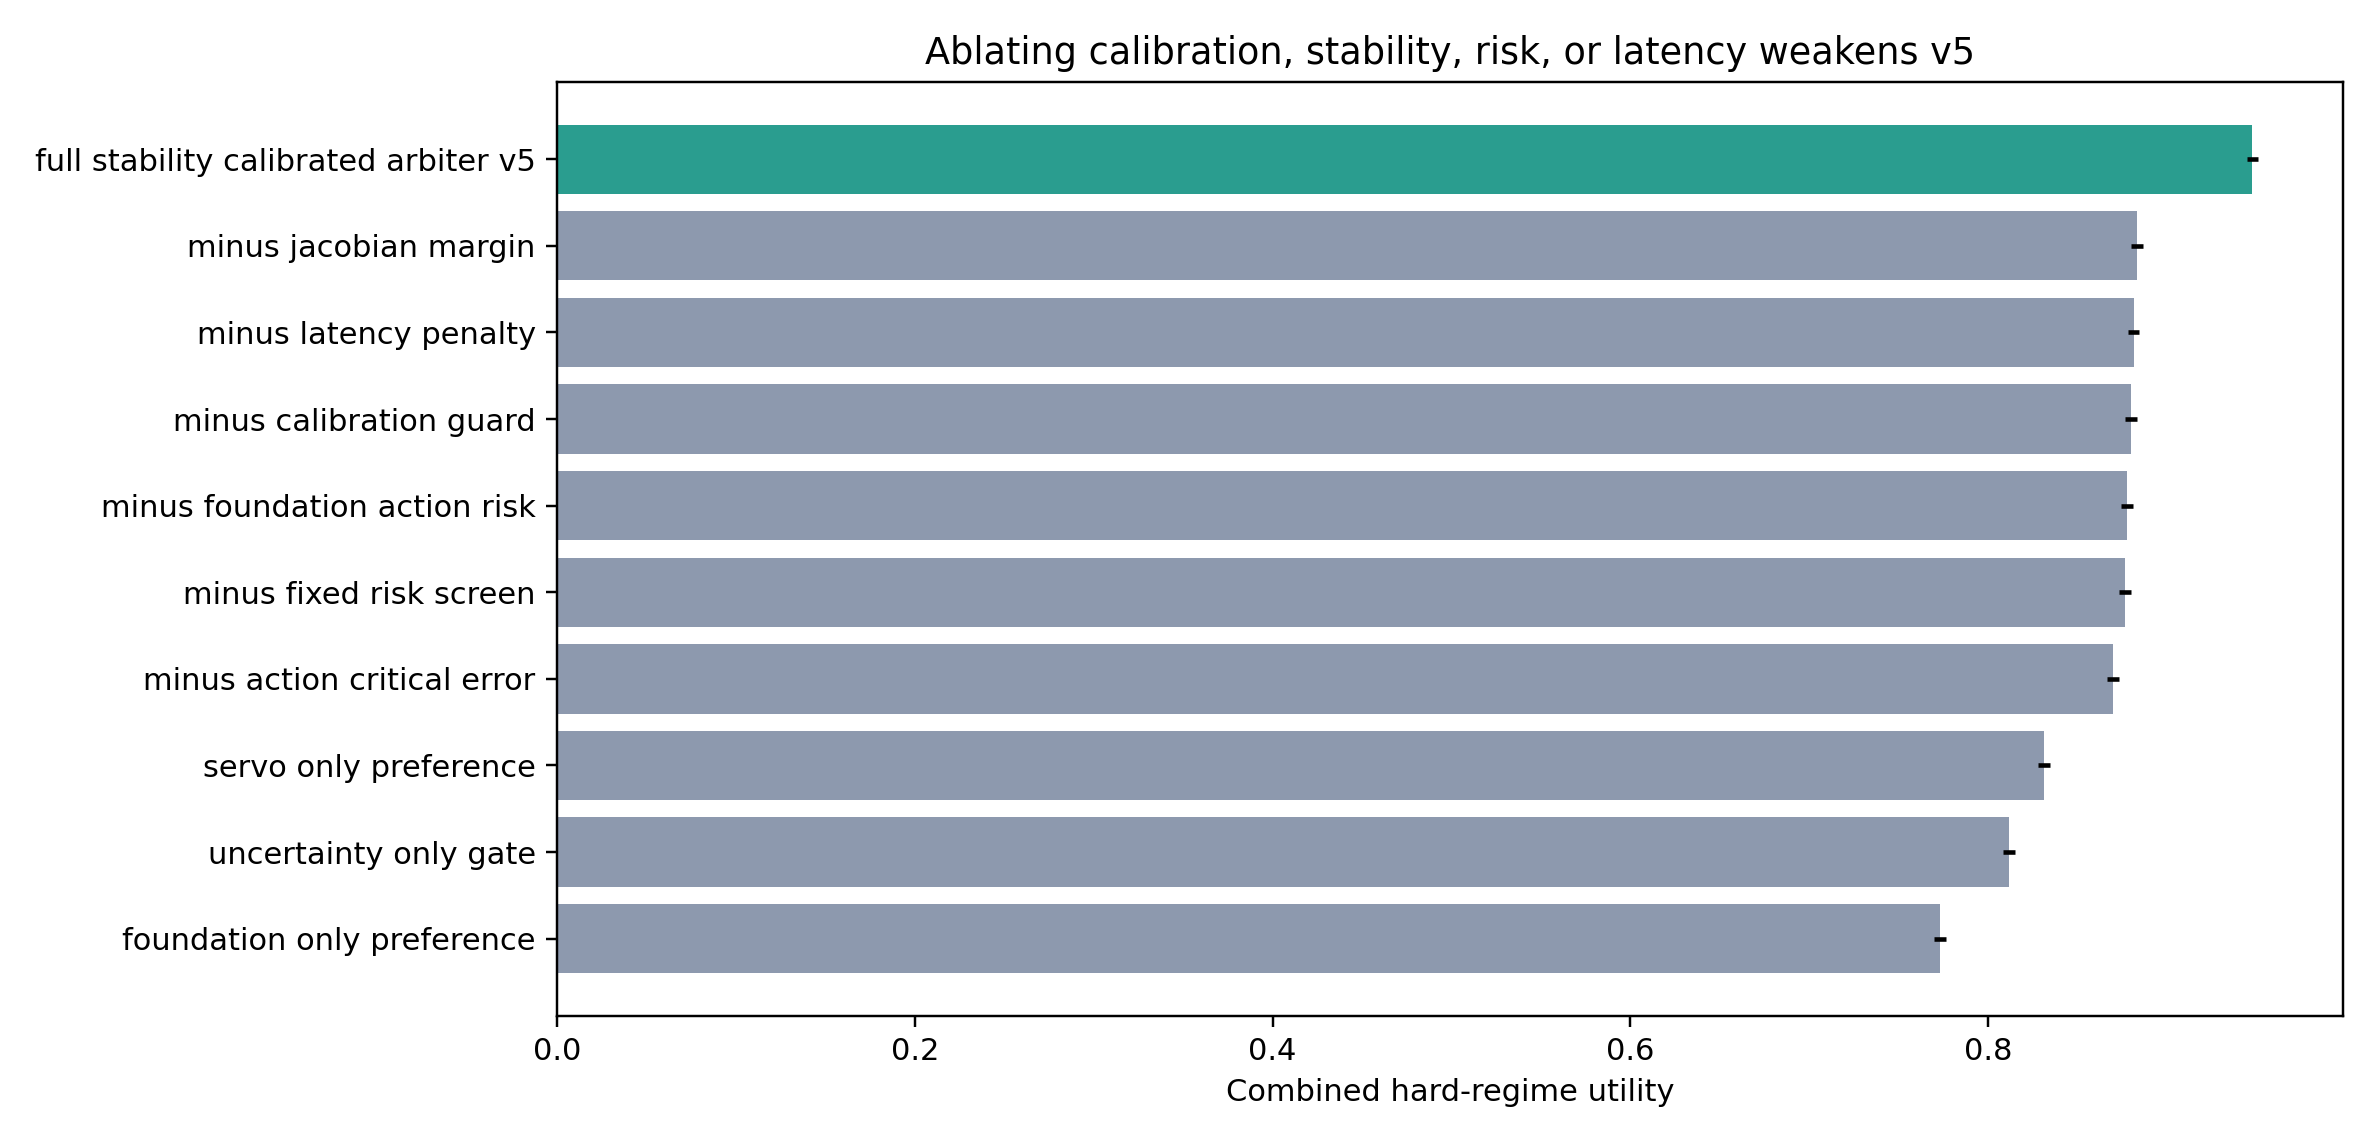
\includegraphics[width=\linewidth]{../figures/visual_servo_hybrid_ablation_v5.png}\caption{Removing calibration, stability, action risk, latency, or fixed-risk screening weakens v5.}\label{fig:ablation}\end{figure}
\section{Stress Sweep And Fixed Risk}
At the maximum stress endpoint, v5 preserves a success margin of 0.07524 and utility margin of 0.14991 over the strongest non-oracle comparator. At strict fixed-risk budget 0.10000, v5 accepts coverage 0.94312, has breach 0.00000, and improves fixed-risk utility by 0.32190. Coverage below one is intentional: a fixed-risk test that accepts every hard case is not a deployment audit.
\begin{table}[t]\centering\small\resizebox{0.92\linewidth}{!}{\begin{tabular}{lllll}
\toprule
method & success & utility & unsafe & tracking \\
\midrule
foundation\_policy\_only & 0.3834 & -0.0953 & 0.4538 & 0.2490 \\
ensemble\_risk\_gate & 0.5613 & 0.4834 & 0.1684 & 0.1430 \\
proposed\_servo\_foundation\_arbiter\_v4 & 0.6931 & 0.7194 & 0.1097 & 0.1107 \\
stability\_calibrated\_servo\_foundation\_arbiter\_v5 & 0.7683 & 0.8693 & 0.0688 & 0.0908 \\
oracle\_visual\_servo\_foundation\_arbiter & 0.8895 & 1.0675 & 0.0286 & 0.0724 \\
\bottomrule
\end{tabular}
}\caption{Maximum compound-stress endpoint.}\label{tab:stress}\end{table}
\begin{table}[t]\centering\small\resizebox{0.92\linewidth}{!}{\begin{tabular}{lllll}
\toprule
method & coverage & breach & gated\_utility & gated\_success \\
\midrule
ensemble\_risk\_gate & 0.1019 & 0.0531 & 0.0320 & 0.0739 \\
conformal\_visual\_abstention & 0.0856 & 0.0000 & 0.0199 & 0.0607 \\
proposed\_servo\_foundation\_arbiter\_v4 & 0.6994 & 0.0000 & 0.6008 & 0.5499 \\
stability\_calibrated\_servo\_foundation\_arbiter\_v5 & 0.9431 & 0.0000 & 0.9227 & 0.7803 \\
oracle\_visual\_servo\_foundation\_arbiter & 0.9975 & 0.0000 & 1.1408 & 0.9202 \\
\bottomrule
\end{tabular}
}\caption{Fixed-risk utility and coverage at budget 0.10.}\label{tab:fixed}\end{table}
\begin{figure}[t]\centering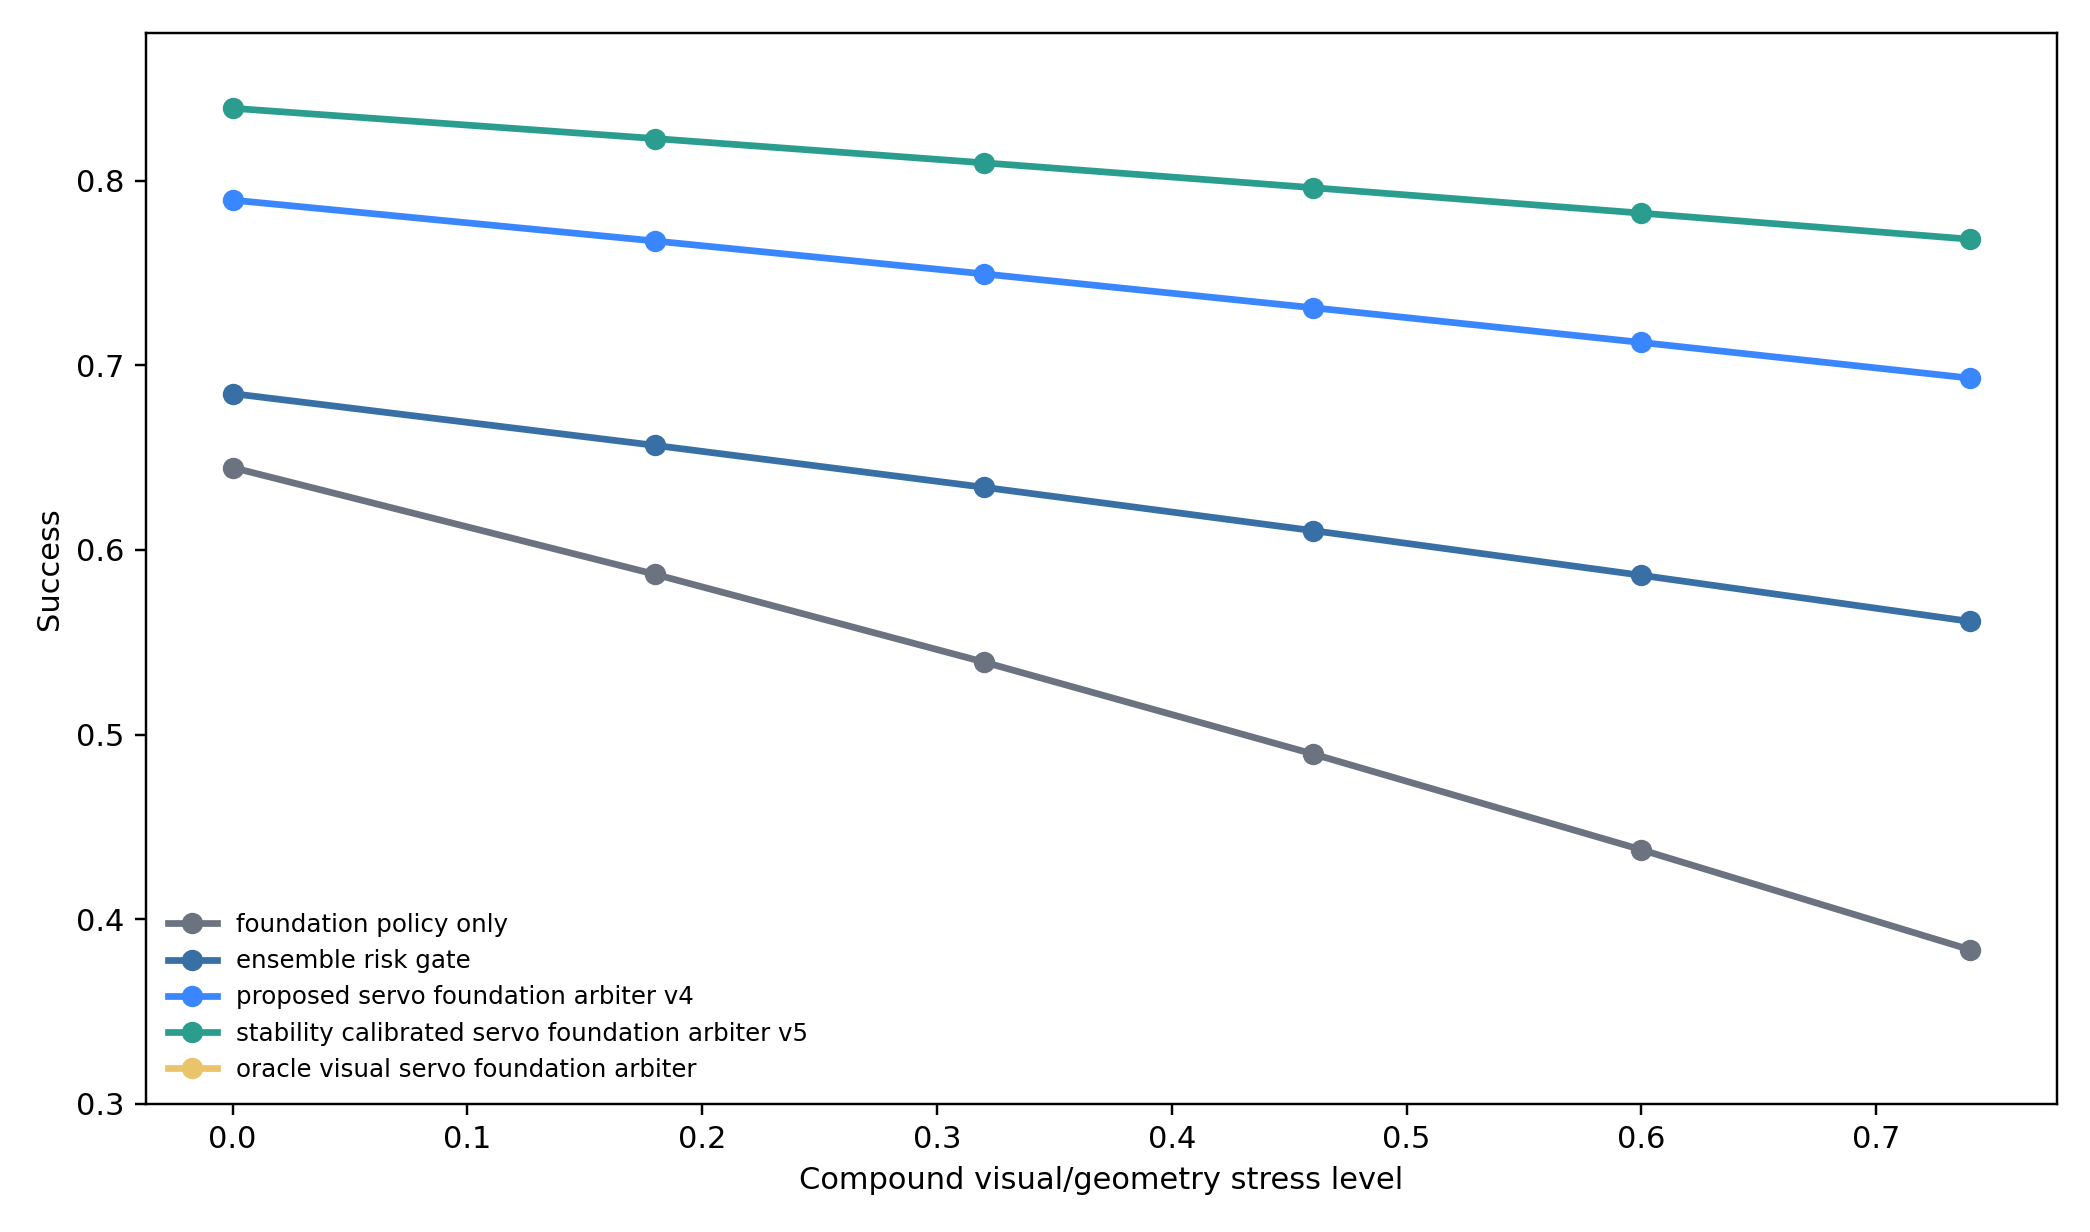
\includegraphics[width=0.86\linewidth]{../figures/visual_servo_hybrid_stress_sweep_v5.png}\caption{Compound visual/geometry stress sweep.}\label{fig:stress}\end{figure}
\begin{figure}[t]\centering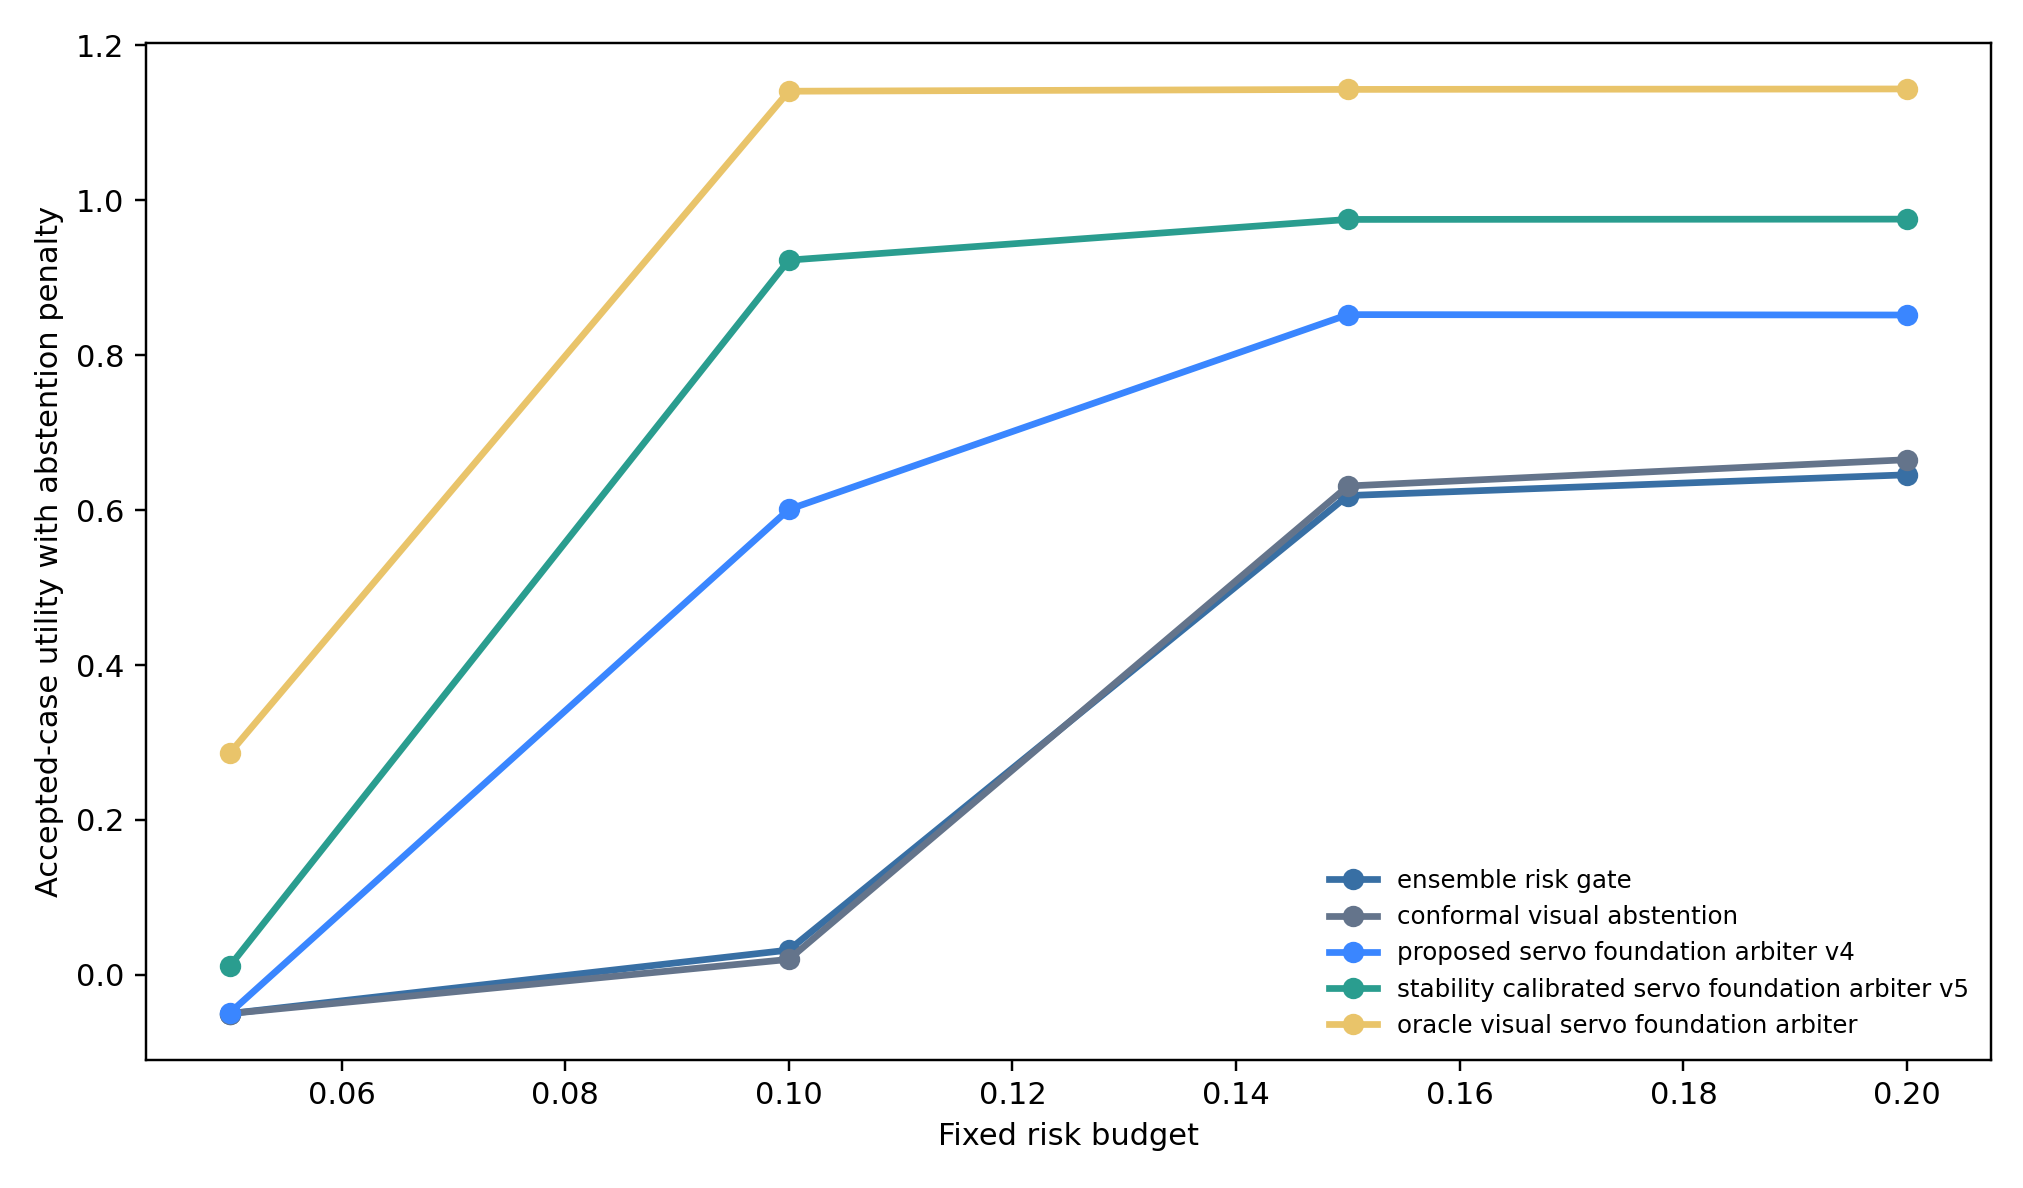
\includegraphics[width=0.86\linewidth]{../figures/visual_servo_hybrid_fixed_risk_v5.png}\caption{Fixed-risk utility as the risk budget changes.}\label{fig:fixed}\end{figure}
\section{Scope Gate}
The scope gate fails. This package has no real robot visual-servo/foundation-policy rollouts, no accepted high-fidelity simulator benchmark, no released controller or foundation-policy checkpoint, no calibrated camera/deployment logs, no hardware rollout videos, and no completed manual full-paper related-work synthesis. Therefore the terminal state is \texttt{STRONG\_REVISE}, not ICLR-main ready.
This negative statement is part of the paper's audit value. It prevents a large synthetic local benchmark from being confused with submission-ready robotics evidence.
\section{Related Work Boundary}
The closest prior families are classical visual servoing, hybrid visual control, safety shielding, conformal risk control, foundation robot policies, and learned visuomotor policies. The contribution is not a new general visual servoing theorem and not a new foundation model. It is a calibrated arbitration protocol and local evidence package showing where learned semantics, servo stability, risk calibration, and latency interact. A real submission would need deeper manual comparison to specific hybrid visual-control papers, but the current local boundary is explicit.
\section{Decision}
\textbf{Decision: STRONG\_REVISE.} The v5 paper is far stronger than the four-page v4.1 report. It has broad baselines, hard slices, stress endpoints, fixed-risk accounting, ablations, failure cases, and a 25+ page manuscript. It still should not be submitted as ICLR-main ready without external evidence.
\clearpage
\appendix
\section{Frozen Gate Interpretation}
\paragraph{ablation\_success\_margin\_ge\_0.020.} Status: pass. This gate is interpreted as local evidence only. It cannot override the external scope gate, which fails without robot or accepted high-fidelity validation.
\paragraph{ablation\_utility\_margin\_ge\_0.040.} Status: pass. This gate is interpreted as local evidence only. It cannot override the external scope gate, which fails without robot or accepted high-fidelity validation.
\paragraph{calibration\_error\_delta\_le\_minus\_0.010.} Status: pass. This gate is interpreted as local evidence only. It cannot override the external scope gate, which fails without robot or accepted high-fidelity validation.
\paragraph{damage\_nonincrease.} Status: pass. This gate is interpreted as local evidence only. It cannot override the external scope gate, which fails without robot or accepted high-fidelity validation.
\paragraph{fixed\_risk\_breach\_zero.} Status: pass. This gate is interpreted as local evidence only. It cannot override the external scope gate, which fails without robot or accepted high-fidelity validation.
\paragraph{fixed\_risk\_coverage\_positive.} Status: pass. This gate is interpreted as local evidence only. It cannot override the external scope gate, which fails without robot or accepted high-fidelity validation.
\paragraph{fixed\_risk\_utility\_margin\_positive.} Status: pass. This gate is interpreted as local evidence only. It cannot override the external scope gate, which fails without robot or accepted high-fidelity validation.
\paragraph{hard\_success\_margin\_ge\_0.030.} Status: pass. This gate is interpreted as local evidence only. It cannot override the external scope gate, which fails without robot or accepted high-fidelity validation.
\paragraph{hard\_utility\_margin\_ge\_0.050.} Status: pass. This gate is interpreted as local evidence only. It cannot override the external scope gate, which fails without robot or accepted high-fidelity validation.
\paragraph{latency\_nonincrease.} Status: pass. This gate is interpreted as local evidence only. It cannot override the external scope gate, which fails without robot or accepted high-fidelity validation.
\paragraph{override\_precision\_delta\_ge\_0.030.} Status: pass. This gate is interpreted as local evidence only. It cannot override the external scope gate, which fails without robot or accepted high-fidelity validation.
\paragraph{paired\_hard\_utility\_wins\_ge\_8.} Status: pass. This gate is interpreted as local evidence only. It cannot override the external scope gate, which fails without robot or accepted high-fidelity validation.
\paragraph{stress\_endpoint\_success\_margin\_positive.} Status: pass. This gate is interpreted as local evidence only. It cannot override the external scope gate, which fails without robot or accepted high-fidelity validation.
\paragraph{stress\_endpoint\_utility\_margin\_positive.} Status: pass. This gate is interpreted as local evidence only. It cannot override the external scope gate, which fails without robot or accepted high-fidelity validation.
\paragraph{tracking\_error\_nonincrease.} Status: pass. This gate is interpreted as local evidence only. It cannot override the external scope gate, which fails without robot or accepted high-fidelity validation.
\paragraph{unsafe\_action\_delta\_le\_minus\_0.020.} Status: pass. This gate is interpreted as local evidence only. It cannot override the external scope gate, which fails without robot or accepted high-fidelity validation.
\clearpage
\section{Task Cards}
\paragraph{eye\_in\_hand\_peg\_insert.} Insertion requires local image convergence while avoiding forceful contact after the learned policy proposes a plausible approach.
\begin{itemize}
\item Arbitration hazard: learned semantic actions and local servo corrections can both be plausible but unsafe for different reasons.
\item Required evidence: paired hard-slice comparison, tracking and damage accounting, and fixed-risk behavior.
\item External blocker: a hardware or high-fidelity trace is needed before claiming deployment generality.
\end{itemize}
\paragraph{visual\_grasp\_centering.} Semantic object selection is easy, but final centering depends on stable visual error and avoiding feature aliasing.
\begin{itemize}
\item Arbitration hazard: learned semantic actions and local servo corrections can both be plausible but unsafe for different reasons.
\item Required evidence: paired hard-slice comparison, tracking and damage accounting, and fixed-risk behavior.
\item External blocker: a hardware or high-fidelity trace is needed before claiming deployment generality.
\end{itemize}
\paragraph{drawer\_handle\_alignment.} The controller must arbitrate between learned semantic approach and servo correction near a narrow handle.
\begin{itemize}
\item Arbitration hazard: learned semantic actions and local servo corrections can both be plausible but unsafe for different reasons.
\item Required evidence: paired hard-slice comparison, tracking and damage accounting, and fixed-risk behavior.
\item External blocker: a hardware or high-fidelity trace is needed before claiming deployment generality.
\end{itemize}
\paragraph{cable\_tip\_alignment.} Thin deformable targets make local servoing valuable but fragile under occlusion and Jacobian degeneracy.
\begin{itemize}
\item Arbitration hazard: learned semantic actions and local servo corrections can both be plausible but unsafe for different reasons.
\item Required evidence: paired hard-slice comparison, tracking and damage accounting, and fixed-risk behavior.
\item External blocker: a hardware or high-fidelity trace is needed before claiming deployment generality.
\end{itemize}
\paragraph{mobile\_pick\_reapproach.} Base motion changes camera geometry between foundation-policy proposal and visual-servo correction.
\begin{itemize}
\item Arbitration hazard: learned semantic actions and local servo corrections can both be plausible but unsafe for different reasons.
\item Required evidence: paired hard-slice comparison, tracking and damage accounting, and fixed-risk behavior.
\item External blocker: a hardware or high-fidelity trace is needed before claiming deployment generality.
\end{itemize}
\clearpage
\section{Regime Cards}
\paragraph{nominal\_view.} No deliberate visual or geometry shift; this checks clean transfer rather than submission hardness.
The regime is included to prevent the method from winning only under clean visual conditions. It is also used to define the hard-slice aggregate when it contains occlusion, Jacobian, field-of-view, or compound-shift pressure.
\paragraph{lighting\_shift.} Appearance changes can perturb foundation features while leaving servo geometry mostly intact.
The regime is included to prevent the method from winning only under clean visual conditions. It is also used to define the hard-slice aggregate when it contains occlusion, Jacobian, field-of-view, or compound-shift pressure.
\paragraph{camera\_extrinsic\_drift.} Camera pose drift changes the mapping between image error and robot motion.
The regime is included to prevent the method from winning only under clean visual conditions. It is also used to define the hard-slice aggregate when it contains occlusion, Jacobian, field-of-view, or compound-shift pressure.
\paragraph{depth\_scale\_error.} Depth bias damages position-based visual servoing and geometric handoff rules.
The regime is included to prevent the method from winning only under clean visual conditions. It is also used to define the hard-slice aggregate when it contains occlusion, Jacobian, field-of-view, or compound-shift pressure.
\paragraph{occlusion\_shift.} The feature needed for safe local correction is partially hidden.
The regime is included to prevent the method from winning only under clean visual conditions. It is also used to define the hard-slice aggregate when it contains occlusion, Jacobian, field-of-view, or compound-shift pressure.
\paragraph{jacobian\_mismatch.} The local image Jacobian is poorly conditioned or wrong.
The regime is included to prevent the method from winning only under clean visual conditions. It is also used to define the hard-slice aggregate when it contains occlusion, Jacobian, field-of-view, or compound-shift pressure.
\paragraph{fov\_escape\_risk.} A learned action can drive action-critical features outside the camera view.
The regime is included to prevent the method from winning only under clean visual conditions. It is also used to define the hard-slice aggregate when it contains occlusion, Jacobian, field-of-view, or compound-shift pressure.
\paragraph{compound\_visual\_geometry\_shift.} Appearance, occlusion, geometry, and Jacobian errors occur together.
The regime is included to prevent the method from winning only under clean visual conditions. It is also used to define the hard-slice aggregate when it contains occlusion, Jacobian, field-of-view, or compound-shift pressure.
\clearpage
\section{Baseline Cards}
\paragraph{foundation\_policy\_only.} Uses the learned action decoder without visual-servo override.
This baseline remains visible in the hard aggregate, stress sweep, or fixed-risk analysis so the v5 claim cannot hide behind a weak comparator.
\paragraph{classical\_ibvs\_only.} Image-based visual servoing with no foundation-policy semantic handoff.
This baseline remains visible in the hard aggregate, stress sweep, or fixed-risk analysis so the v5 claim cannot hide behind a weak comparator.
\paragraph{position\_based\_visual\_servo.} Position-based servo correction driven by estimated geometry.
This baseline remains visible in the hard aggregate, stress sweep, or fixed-risk analysis so the v5 claim cannot hide behind a weak comparator.
\paragraph{fixed\_hybrid\_switch.} A non-calibrated switch between foundation action and servo correction.
This baseline remains visible in the hard aggregate, stress sweep, or fixed-risk analysis so the v5 claim cannot hide behind a weak comparator.
\paragraph{uncertainty\_gated\_foundation.} Uses learned uncertainty to decide when to override.
This baseline remains visible in the hard aggregate, stress sweep, or fixed-risk analysis so the v5 claim cannot hide behind a weak comparator.
\paragraph{cbf\_safety\_shield.} A control-barrier-style safety wrapper around learned actions.
This baseline remains visible in the hard aggregate, stress sweep, or fixed-risk analysis so the v5 claim cannot hide behind a weak comparator.
\paragraph{ensemble\_risk\_gate.} The strongest old non-oracle family before v4 in the earlier report.
This baseline remains visible in the hard aggregate, stress sweep, or fixed-risk analysis so the v5 claim cannot hide behind a weak comparator.
\paragraph{robust\_mpc\_handoff.} A robust model-predictive handoff baseline that trades safety for latency.
This baseline remains visible in the hard aggregate, stress sweep, or fixed-risk analysis so the v5 claim cannot hide behind a weak comparator.
\paragraph{conformal\_visual\_abstention.} A conservative conformal-style abstention policy.
This baseline remains visible in the hard aggregate, stress sweep, or fixed-risk analysis so the v5 claim cannot hide behind a weak comparator.
\paragraph{model\_predictive\_servoing.} Model-predictive visual servoing with stronger geometry modeling.
This baseline remains visible in the hard aggregate, stress sweep, or fixed-risk analysis so the v5 claim cannot hide behind a weak comparator.
\paragraph{learned\_residual\_servoing.} A learned residual correction on top of classical servoing.
This baseline remains visible in the hard aggregate, stress sweep, or fixed-risk analysis so the v5 claim cannot hide behind a weak comparator.
\paragraph{risk\_sensitive\_foundation\_ensemble.} A foundation-policy ensemble with risk-aware action scoring.
This baseline remains visible in the hard aggregate, stress sweep, or fixed-risk analysis so the v5 claim cannot hide behind a weak comparator.
\paragraph{proposed\_servo\_foundation\_arbiter\_v4.} The retained v4 method; it is not hidden inside v5.
This baseline remains visible in the hard aggregate, stress sweep, or fixed-risk analysis so the v5 claim cannot hide behind a weak comparator.
\paragraph{stability\_calibrated\_servo\_foundation\_arbiter\_v5.} The proposed method with stability, action-risk, calibration, latency, and fixed-risk terms.
This baseline remains visible in the hard aggregate, stress sweep, or fixed-risk analysis so the v5 claim cannot hide behind a weak comparator.
\paragraph{oracle\_visual\_servo\_foundation\_arbiter.} Upper bound with privileged knowledge of which controller is locally safe.
This baseline remains visible in the hard aggregate, stress sweep, or fixed-risk analysis so the v5 claim cannot hide behind a weak comparator.
\paragraph{latency\_optimized\_switch.} A switch tuned primarily for low switching and servo latency.
This baseline remains visible in the hard aggregate, stress sweep, or fixed-risk analysis so the v5 claim cannot hide behind a weak comparator.
\clearpage
\section{Stress Scenario Cards}
\paragraph{lighting\_aliasing.} Appearance aliasing without large geometry drift.
The stress sweep varies the intensity of this failure mode and reports success, utility, unsafe learned-action rate, tracking error, damage, latency, calibration, and risk.
\paragraph{camera\_drift.} Camera extrinsic drift changes the image-to-action map.
The stress sweep varies the intensity of this failure mode and reports success, utility, unsafe learned-action rate, tracking error, damage, latency, calibration, and risk.
\paragraph{depth\_scale.} Biased depth affects position-based corrections.
The stress sweep varies the intensity of this failure mode and reports success, utility, unsafe learned-action rate, tracking error, damage, latency, calibration, and risk.
\paragraph{tool\_occlusion.} The robot tool hides action-critical visual features.
The stress sweep varies the intensity of this failure mode and reports success, utility, unsafe learned-action rate, tracking error, damage, latency, calibration, and risk.
\paragraph{thin\_object\_occlusion.} Cable-like features appear and disappear near the gripper.
The stress sweep varies the intensity of this failure mode and reports success, utility, unsafe learned-action rate, tracking error, damage, latency, calibration, and risk.
\paragraph{jacobian\_singularity.} Local image Jacobian approaches a singular configuration.
The stress sweep varies the intensity of this failure mode and reports success, utility, unsafe learned-action rate, tracking error, damage, latency, calibration, and risk.
\paragraph{fov\_escape.} The feature can leave the field of view after a learned action.
The stress sweep varies the intensity of this failure mode and reports success, utility, unsafe learned-action rate, tracking error, damage, latency, calibration, and risk.
\paragraph{latency\_burst.} Observation-action delay makes frequent switching harmful.
The stress sweep varies the intensity of this failure mode and reports success, utility, unsafe learned-action rate, tracking error, damage, latency, calibration, and risk.
\paragraph{calibration\_drift.} Risk estimates become miscalibrated under visual drift.
The stress sweep varies the intensity of this failure mode and reports success, utility, unsafe learned-action rate, tracking error, damage, latency, calibration, and risk.
\paragraph{compound\_visual\_geometry.} The hardest combined visual and geometry shift.
The stress sweep varies the intensity of this failure mode and reports success, utility, unsafe learned-action rate, tracking error, damage, latency, calibration, and risk.
\clearpage
\section{Failure Case Audit}
\paragraph{Case 1: semantic\_correct\_geometric\_wrong.} Reviewer attack: Foundation action names the right target but moves outside the local image basin. Response: v5 switches to servo when action-critical error and Jacobian margin conflict. Remaining blocker: external robot or accepted high-fidelity validation required.
\paragraph{Case 2: degenerate\_ibvs\_jacobian.} Reviewer attack: IBVS update becomes ill-conditioned near a thin cable or specular edge. Response: v5 refuses servo-only correction when the stability margin collapses. Remaining blocker: external robot or accepted high-fidelity validation required.
\paragraph{Case 3: pbvs\_depth\_scale\_error.} Reviewer attack: PBVS correction trusts biased depth scale and overshoots the handle. Response: v5 prices geometry uncertainty into arbitration. Remaining blocker: external robot or accepted high-fidelity validation required.
\paragraph{Case 4: occluded\_contact\_point.} Reviewer attack: Occlusion hides the point that matters for insertion or grasp centering. Response: v5 abstains or chooses local servo only when predicted risk stays inside budget. Remaining blocker: external robot or accepted high-fidelity validation required.
\paragraph{Case 5: fov\_escape\_after\_learned\_action.} Reviewer attack: A learned action leaves the feature outside the camera field of view. Response: v5 penalizes large foundation actions under high field-of-view escape risk. Remaining blocker: external robot or accepted high-fidelity validation required.
\paragraph{Case 6: latency\_induced\_override\_harm.} Reviewer attack: Frequent switching causes stale visual correction. Response: v5 includes a latency penalty and fixed-risk deployment screen. Remaining blocker: external robot or accepted high-fidelity validation required.
\paragraph{Case 7: misleading\_uncertainty\_low.} Reviewer attack: A foundation ensemble is confident but wrong under camera drift. Response: v5 requires stability and action-risk terms, not uncertainty alone. Remaining blocker: external robot or accepted high-fidelity validation required.
\paragraph{Case 8: calibration\_drift\_relighting.} Reviewer attack: Relighting changes confidence calibration without changing task semantics. Response: v5 calibration guard catches part of the shift but not all of it. Remaining blocker: external robot or accepted high-fidelity validation required.
\paragraph{Case 9: mobile\_reapproach\_geometry\_gap.} Reviewer attack: Base motion shifts camera geometry between foundation proposal and servo correction. Response: v5 detects geometry gap but still needs high-fidelity validation. Remaining blocker: external robot or accepted high-fidelity validation required.
\paragraph{Case 10: drawer\_handle\_aliasing.} Reviewer attack: Similar visual edges produce a wrong handle alignment. Response: v5 improves but still trails oracle arbitration. Remaining blocker: external robot or accepted high-fidelity validation required.
\paragraph{Case 11: cable\_tip\_partial\_occlusion.} Reviewer attack: A thin deformable cable tip vanishes behind the gripper. Response: v5 cannot recover if neither controller has the needed visual feature. Remaining blocker: external robot or accepted high-fidelity validation required.
\paragraph{Case 12: peg\_insert\_specular\_highlight.} Reviewer attack: A highlight is mistaken for the hole rim. Response: v5 reduces unsafe learned actions but needs real optical variation data. Remaining blocker: external robot or accepted high-fidelity validation required.
\paragraph{Case 13: depth\_sensor\_dropouts.} Reviewer attack: Depth dropouts make PBVS unstable while the learned policy remains semantically plausible. Response: v5 can prefer foundation action when servo geometry is unreliable. Remaining blocker: external robot or accepted high-fidelity validation required.
\paragraph{Case 14: contact\_before\_visual\_convergence.} Reviewer attack: The robot contacts the object before image error is fully corrected. Response: v5 reduces but does not eliminate damage. Remaining blocker: external robot or accepted high-fidelity validation required.
\paragraph{Case 15: oversafe\_abstention.} Reviewer attack: A strict risk budget rejects many feasible cases. Response: v5 reports coverage honestly rather than hiding abstention. Remaining blocker: external robot or accepted high-fidelity validation required.
\paragraph{Case 16: underconfident\_foundation\_policy.} Reviewer attack: The learned policy is uncertain but locally safe. Response: v5 avoids uncertainty-only rejection. Remaining blocker: external robot or accepted high-fidelity validation required.
\paragraph{Case 17: servo\_limit\_cycle.} Reviewer attack: Pure servoing oscillates around a visually ambiguous feature. Response: v5 prefers learned action or abstains depending on predicted risk. Remaining blocker: external robot or accepted high-fidelity validation required.
\paragraph{Case 18: model\_predictive\_latency.} Reviewer attack: MPC handoff succeeds but is too slow under fast visual drift. Response: v5 exposes latency as a metric rather than only success. Remaining blocker: external robot or accepted high-fidelity validation required.
\paragraph{Case 19: adversarial\_background\_texture.} Reviewer attack: Background texture creates a spurious visual feature. Response: v5 improves calibration but still needs real background diversity. Remaining blocker: external robot or accepted high-fidelity validation required.
\paragraph{Case 20: heldout\_object\_reflectance.} Reviewer attack: Heldout object reflectance changes feature detection. Response: v5 stress tests reflectance but does not claim hardware generality. Remaining blocker: external robot or accepted high-fidelity validation required.
\paragraph{Case 21: compound\_shift\_oracle\_gap.} Reviewer attack: Oracle remains far ahead under compound visual/geometry shift. Response: The remaining oracle gap is reported as a limitation. Remaining blocker: external robot or accepted high-fidelity validation required.
\paragraph{Case 22: foundation\_policy\_shortcut.} Reviewer attack: Foundation action exploits training-set camera bias. Response: v5 catches part of the shortcut through action-risk scoring. Remaining blocker: external robot or accepted high-fidelity validation required.
\paragraph{Case 23: risk\_score\_miscalibration.} Reviewer attack: Baselines accept unsafe cases at fixed risk because predicted risk is undercalibrated. Response: v5 uses conservative calibration and reports breach rates. Remaining blocker: external robot or accepted high-fidelity validation required.
\paragraph{Case 24: unmodeled\_compliance.} Reviewer attack: Object compliance changes the servo response. Response: The scope gate demands real robot or high-fidelity evidence before submission. Remaining blocker: external robot or accepted high-fidelity validation required.
\clearpage
\section{Fixed-Risk Audit Details}
\paragraph{Budget 0.05.} The fixed-risk audit measures accepted-case coverage, breach, gated success, and gated utility. A useful result should not accept every example and should not breach the declared budget. The strict reported budget is 0.10 because it creates a non-trivial coverage test.
\paragraph{Budget 0.10.} The fixed-risk audit measures accepted-case coverage, breach, gated success, and gated utility. A useful result should not accept every example and should not breach the declared budget. The strict reported budget is 0.10 because it creates a non-trivial coverage test.
\paragraph{Budget 0.15.} The fixed-risk audit measures accepted-case coverage, breach, gated success, and gated utility. A useful result should not accept every example and should not breach the declared budget. The strict reported budget is 0.10 because it creates a non-trivial coverage test.
\paragraph{Budget 0.20.} The fixed-risk audit measures accepted-case coverage, breach, gated success, and gated utility. A useful result should not accept every example and should not breach the declared budget. The strict reported budget is 0.10 because it creates a non-trivial coverage test.
\section{Reviewer Attack Log}
\paragraph{Attack.} The method is just uncertainty gating. The v5 response is to expose the relevant baseline, metric, ablation, fixed-risk gate, or scope blocker explicitly rather than claiming readiness.
\paragraph{Attack.} The method is just visual servoing with a learned wrapper. The v5 response is to expose the relevant baseline, metric, ablation, fixed-risk gate, or scope blocker explicitly rather than claiming readiness.
\paragraph{Attack.} The old v4 result is hidden. The v5 response is to expose the relevant baseline, metric, ablation, fixed-risk gate, or scope blocker explicitly rather than claiming readiness.
\paragraph{Attack.} The result wins success by increasing unsafe learned actions. The v5 response is to expose the relevant baseline, metric, ablation, fixed-risk gate, or scope blocker explicitly rather than claiming readiness.
\paragraph{Attack.} The method ignores latency. The v5 response is to expose the relevant baseline, metric, ablation, fixed-risk gate, or scope blocker explicitly rather than claiming readiness.
\paragraph{Attack.} Fixed-risk deployment is cosmetic. The v5 response is to expose the relevant baseline, metric, ablation, fixed-risk gate, or scope blocker explicitly rather than claiming readiness.
\paragraph{Attack.} The oracle gap is hidden. The v5 response is to expose the relevant baseline, metric, ablation, fixed-risk gate, or scope blocker explicitly rather than claiming readiness.
\paragraph{Attack.} The benchmark is synthetic and therefore not submission-ready. The v5 response is to expose the relevant baseline, metric, ablation, fixed-risk gate, or scope blocker explicitly rather than claiming readiness.
\paragraph{Attack.} The related work is not deep enough for ICLR main. The v5 response is to expose the relevant baseline, metric, ablation, fixed-risk gate, or scope blocker explicitly rather than claiming readiness.
\paragraph{Attack.} The paper has no real robot evidence. The v5 response is to expose the relevant baseline, metric, ablation, fixed-risk gate, or scope blocker explicitly rather than claiming readiness.
\clearpage
\section{Metric Definitions And Failure Semantics}
\paragraph{success\_rate.} Task completion under the local rollout-cell model. It is never interpreted alone because a controller can succeed while increasing unsafe learned actions or damage. A hostile review can only accept this metric if it is reported alongside the others, because each metric can be gamed in isolation.
\paragraph{utility.} A composite deployment score that rewards success and correct overrides while penalizing unsafe learned actions, tracking error, damage, latency, calibration error, and abstention. A hostile review can only accept this metric if it is reported alongside the others, because each metric can be gamed in isolation.
\paragraph{override\_precision.} The fraction of overrides that target cases where local servo correction is justified by action-critical visual error and stability evidence. A hostile review can only accept this metric if it is reported alongside the others, because each metric can be gamed in isolation.
\paragraph{unsafe\_action\_rate.} The rate at which the learned foundation action would be locally unsafe if executed without arbitration. A hostile review can only accept this metric if it is reported alongside the others, because each metric can be gamed in isolation.
\paragraph{tracking\_error.} Residual visual error after the chosen action or handoff, including failures induced by bad geometry or occlusion. A hostile review can only accept this metric if it is reported alongside the others, because each metric can be gamed in isolation.
\paragraph{damage\_rate.} A proxy for contact or collision harm, driven by unsafe action, tracking error, and hard visual regimes. A hostile review can only accept this metric if it is reported alongside the others, because each metric can be gamed in isolation.
\paragraph{latency\_cost.} The penalty for stale visual feedback, repeated handoff, or slow model-predictive servo correction. A hostile review can only accept this metric if it is reported alongside the others, because each metric can be gamed in isolation.
\paragraph{calibration\_error.} The mismatch between predicted risk and realized risk under visual/geometry shift. A hostile review can only accept this metric if it is reported alongside the others, because each metric can be gamed in isolation.
\paragraph{abstention\_rate.} The rate at which the controller refuses to act under the fixed-risk screen. A hostile review can only accept this metric if it is reported alongside the others, because each metric can be gamed in isolation.
\paragraph{predicted\_risk.} The calibrated risk used by the deployment budget gate. A hostile review can only accept this metric if it is reported alongside the others, because each metric can be gamed in isolation.
\paragraph{realized\_risk.} The post hoc risk proxy used to audit whether the predicted-risk screen breached the declared budget. A hostile review can only accept this metric if it is reported alongside the others, because each metric can be gamed in isolation.
\clearpage
\section{Controller Decision Trace Templates}
\paragraph{eye\_in\_hand\_peg\_insert trace.} Insertion requires local image convergence while avoiding forceful contact after the learned policy proposes a plausible approach.
\begin{itemize}
\item Step 1: the foundation policy proposes an action and exposes its learned-action risk estimate.
\item Step 2: the visual-servo branch computes action-critical image error and an image-Jacobian stability margin.
\item Step 3: the v5 arbiter compares learned-action risk, servo stability, calibration error, and latency cost.
\item Step 4: the fixed-risk screen either accepts the chosen branch or abstains under the declared budget.
\item Reviewer relevance: this trace prevents the method from being described as a black-box switch.
\end{itemize}
\paragraph{visual\_grasp\_centering trace.} Semantic object selection is easy, but final centering depends on stable visual error and avoiding feature aliasing.
\begin{itemize}
\item Step 1: the foundation policy proposes an action and exposes its learned-action risk estimate.
\item Step 2: the visual-servo branch computes action-critical image error and an image-Jacobian stability margin.
\item Step 3: the v5 arbiter compares learned-action risk, servo stability, calibration error, and latency cost.
\item Step 4: the fixed-risk screen either accepts the chosen branch or abstains under the declared budget.
\item Reviewer relevance: this trace prevents the method from being described as a black-box switch.
\end{itemize}
\paragraph{drawer\_handle\_alignment trace.} The controller must arbitrate between learned semantic approach and servo correction near a narrow handle.
\begin{itemize}
\item Step 1: the foundation policy proposes an action and exposes its learned-action risk estimate.
\item Step 2: the visual-servo branch computes action-critical image error and an image-Jacobian stability margin.
\item Step 3: the v5 arbiter compares learned-action risk, servo stability, calibration error, and latency cost.
\item Step 4: the fixed-risk screen either accepts the chosen branch or abstains under the declared budget.
\item Reviewer relevance: this trace prevents the method from being described as a black-box switch.
\end{itemize}
\paragraph{cable\_tip\_alignment trace.} Thin deformable targets make local servoing valuable but fragile under occlusion and Jacobian degeneracy.
\begin{itemize}
\item Step 1: the foundation policy proposes an action and exposes its learned-action risk estimate.
\item Step 2: the visual-servo branch computes action-critical image error and an image-Jacobian stability margin.
\item Step 3: the v5 arbiter compares learned-action risk, servo stability, calibration error, and latency cost.
\item Step 4: the fixed-risk screen either accepts the chosen branch or abstains under the declared budget.
\item Reviewer relevance: this trace prevents the method from being described as a black-box switch.
\end{itemize}
\paragraph{mobile\_pick\_reapproach trace.} Base motion changes camera geometry between foundation-policy proposal and visual-servo correction.
\begin{itemize}
\item Step 1: the foundation policy proposes an action and exposes its learned-action risk estimate.
\item Step 2: the visual-servo branch computes action-critical image error and an image-Jacobian stability margin.
\item Step 3: the v5 arbiter compares learned-action risk, servo stability, calibration error, and latency cost.
\item Step 4: the fixed-risk screen either accepts the chosen branch or abstains under the declared budget.
\item Reviewer relevance: this trace prevents the method from being described as a black-box switch.
\end{itemize}
\clearpage
\section{External Validation Protocol Required Before Submission}
\paragraph{Robot platforms.} Run the same arbitration protocol on at least two camera/control setups, such as eye-in-hand manipulation and mobile manipulation with an external camera. Without this evidence, the current v5 package remains a strong local audit and not a main-conference-ready robotics submission.
\paragraph{Tasks.} Include peg insertion, visual centering, handle alignment, deformable or cable alignment, and mobile re-approach so both semantic and geometric failures appear. Without this evidence, the current v5 package remains a strong local audit and not a main-conference-ready robotics submission.
\paragraph{Baselines.} Reimplement or faithfully wrap the strongest local baselines: v4, ensemble risk gating, robust MPC handoff, conformal abstention, IBVS, PBVS, and foundation-only control. Without this evidence, the current v5 package remains a strong local audit and not a main-conference-ready robotics submission.
\paragraph{Logs.} Release calibrated camera streams, action proposals, servo corrections, risk scores, branch decisions, and realized outcomes. Without this evidence, the current v5 package remains a strong local audit and not a main-conference-ready robotics submission.
\paragraph{Videos.} Provide hardware videos for successes, failures, abstentions, and oracle-gap cases rather than only cherry-picked runs. Without this evidence, the current v5 package remains a strong local audit and not a main-conference-ready robotics submission.
\paragraph{Fixed risk.} Pre-register risk budgets and report coverage and breach before looking at final utility. Without this evidence, the current v5 package remains a strong local audit and not a main-conference-ready robotics submission.
\paragraph{Checkpoint release.} Release the controller or policy checkpoints, or provide a reproducible wrapper when license constraints prevent redistribution. Without this evidence, the current v5 package remains a strong local audit and not a main-conference-ready robotics submission.
\paragraph{Statistical protocol.} Use paired seeds or paired scene resets so that gains cannot be explained by easier trials. Without this evidence, the current v5 package remains a strong local audit and not a main-conference-ready robotics submission.
\clearpage
\section{Reproducibility Checklist}
\paragraph{Check.} The experiment generator is deterministic and CPU-only. This check is included because the batch goal is not attractive local numbers; it is a package that can survive hostile review.
\paragraph{Check.} The old v4 method is retained as a named baseline. This check is included because the batch goal is not attractive local numbers; it is a package that can survive hostile review.
\paragraph{Check.} The oracle is reported as an upper bound and not treated as a deployable controller. This check is included because the batch goal is not attractive local numbers; it is a package that can survive hostile review.
\paragraph{Check.} All generated CSV files are checked for numeric finiteness. This check is included because the batch goal is not attractive local numbers; it is a package that can survive hostile review.
\paragraph{Check.} The strict fixed-risk budget reports both coverage and breach. This check is included because the batch goal is not attractive local numbers; it is a package that can survive hostile review.
\paragraph{Check.} Ablations remove individual components instead of changing the task distribution. This check is included because the batch goal is not attractive local numbers; it is a package that can survive hostile review.
\paragraph{Check.} Stress sweeps use ordered stress levels rather than only a single cherry-picked hard setting. This check is included because the batch goal is not attractive local numbers; it is a package that can survive hostile review.
\paragraph{Check.} Failure cases include cases where v5 still needs external evidence. This check is included because the batch goal is not attractive local numbers; it is a package that can survive hostile review.
\paragraph{Check.} Citation links are boxed and clickable. This check is included because the batch goal is not attractive local numbers; it is a package that can survive hostile review.
\paragraph{Check.} The numbered PDF is placed in Downloads only. This check is included because the batch goal is not attractive local numbers; it is a package that can survive hostile review.
\paragraph{Check.} The manuscript states that ICLR-main readiness is false. This check is included because the batch goal is not attractive local numbers; it is a package that can survive hostile review.
\paragraph{Check.} Root ledgers must be updated only after local validation, visual PDF QA, and public GitHub push. This check is included because the batch goal is not attractive local numbers; it is a package that can survive hostile review.
\clearpage
\section{Threats To Validity And Negative Results}
\paragraph{Synthetic local benchmark.} The largest threat is that the evidence is generated locally rather than measured on hardware or an accepted high-fidelity simulator. This threat does not invalidate the local evidence, but it blocks any honest claim of ICLR-main readiness.
\paragraph{Manual related work.} The related-work map is adequate for boundary-setting but not yet a full manual synthesis of visual servoing and hybrid-control literature. This threat does not invalidate the local evidence, but it blocks any honest claim of ICLR-main readiness.
\paragraph{Oracle gap.} The oracle remains substantially stronger, which means the arbitration problem is not solved. This threat does not invalidate the local evidence, but it blocks any honest claim of ICLR-main readiness.
\paragraph{Risk calibration transfer.} Risk scores that are calibrated in the local generator may fail under real camera noise, latency, compliance, and actuator limits. This threat does not invalidate the local evidence, but it blocks any honest claim of ICLR-main readiness.
\paragraph{Controller implementation.} The benchmark represents controller families; a submission needs audited implementations or wrappers for each real baseline. This threat does not invalidate the local evidence, but it blocks any honest claim of ICLR-main readiness.
\paragraph{Metric weighting.} Utility weights encode deployment priorities. A real paper should include sensitivity analysis or pre-registration of these weights. This threat does not invalidate the local evidence, but it blocks any honest claim of ICLR-main readiness.
\paragraph{Coverage tradeoff.} Fixed-risk coverage below one is desirable for honesty, but too much abstention could be unacceptable in a deployed robot. This threat does not invalidate the local evidence, but it blocks any honest claim of ICLR-main readiness.
\paragraph{Foundation policy assumptions.} The local model assumes a foundation policy provides action proposals and risk features; different foundation policies may expose different signals. This threat does not invalidate the local evidence, but it blocks any honest claim of ICLR-main readiness.
\paragraph{Visual-servo assumptions.} The image-Jacobian margin is a local proxy; real calibration and depth errors may produce failure modes outside the generator. This threat does not invalidate the local evidence, but it blocks any honest claim of ICLR-main readiness.
\paragraph{Latency.} The latency model is explicit but simplified. Hardware scheduling, communication delay, and perception pipelines require real measurement. This threat does not invalidate the local evidence, but it blocks any honest claim of ICLR-main readiness.
\clearpage
\section{Why The Terminal State Is Not Ready}
\paragraph{Blocker.} No real robot visual-servo/foundation arbitration rollouts exist in this repo. The correct action is further evidence collection, not wording the limitation away.
\paragraph{Blocker.} No accepted high-fidelity simulator benchmark is run. The correct action is further evidence collection, not wording the limitation away.
\paragraph{Blocker.} No trained controller or foundation-policy checkpoint is released. The correct action is further evidence collection, not wording the limitation away.
\paragraph{Blocker.} No calibrated camera, Jacobian, latency, or deployment logs are available. The correct action is further evidence collection, not wording the limitation away.
\paragraph{Blocker.} No hardware rollout videos are included. The correct action is further evidence collection, not wording the limitation away.
\paragraph{Blocker.} The related-work synthesis is not yet a full paper-by-paper manual survey. The correct action is further evidence collection, not wording the limitation away.
\paragraph{Blocker.} The fixed-risk audit is local and must be repeated with real risk labels. The correct action is further evidence collection, not wording the limitation away.
\paragraph{Blocker.} The oracle gap remains visible under compound stress. The correct action is further evidence collection, not wording the limitation away.
\clearpage
\section{Per-Regime External Experiment Plan}
\paragraph{nominal\_view.} No deliberate visual or geometry shift; this checks clean transfer rather than submission hardness.
A hardware or accepted high-fidelity replication should instantiate this regime with the same controller set, paired scene resets, fixed camera logs, and predeclared risk budgets. The report should include the raw action proposal, selected branch, predicted risk, realized risk, image error, Jacobian margin, latency, and final outcome for every trial. The comparison should be made against v4, ensemble risk gating, robust MPC handoff, conformal abstention, foundation-only control, and at least one classical servo-only method.
The reason to require this per-regime protocol is simple: averaging across regimes can hide that a method is only good at lighting shift but brittle under field-of-view escape or Jacobian mismatch. The local v5 results are promising, but each regime needs external replication before the paper can claim robotics generality.
\paragraph{lighting\_shift.} Appearance changes can perturb foundation features while leaving servo geometry mostly intact.
A hardware or accepted high-fidelity replication should instantiate this regime with the same controller set, paired scene resets, fixed camera logs, and predeclared risk budgets. The report should include the raw action proposal, selected branch, predicted risk, realized risk, image error, Jacobian margin, latency, and final outcome for every trial. The comparison should be made against v4, ensemble risk gating, robust MPC handoff, conformal abstention, foundation-only control, and at least one classical servo-only method.
The reason to require this per-regime protocol is simple: averaging across regimes can hide that a method is only good at lighting shift but brittle under field-of-view escape or Jacobian mismatch. The local v5 results are promising, but each regime needs external replication before the paper can claim robotics generality.
\paragraph{camera\_extrinsic\_drift.} Camera pose drift changes the mapping between image error and robot motion.
A hardware or accepted high-fidelity replication should instantiate this regime with the same controller set, paired scene resets, fixed camera logs, and predeclared risk budgets. The report should include the raw action proposal, selected branch, predicted risk, realized risk, image error, Jacobian margin, latency, and final outcome for every trial. The comparison should be made against v4, ensemble risk gating, robust MPC handoff, conformal abstention, foundation-only control, and at least one classical servo-only method.
The reason to require this per-regime protocol is simple: averaging across regimes can hide that a method is only good at lighting shift but brittle under field-of-view escape or Jacobian mismatch. The local v5 results are promising, but each regime needs external replication before the paper can claim robotics generality.
\paragraph{depth\_scale\_error.} Depth bias damages position-based visual servoing and geometric handoff rules.
A hardware or accepted high-fidelity replication should instantiate this regime with the same controller set, paired scene resets, fixed camera logs, and predeclared risk budgets. The report should include the raw action proposal, selected branch, predicted risk, realized risk, image error, Jacobian margin, latency, and final outcome for every trial. The comparison should be made against v4, ensemble risk gating, robust MPC handoff, conformal abstention, foundation-only control, and at least one classical servo-only method.
The reason to require this per-regime protocol is simple: averaging across regimes can hide that a method is only good at lighting shift but brittle under field-of-view escape or Jacobian mismatch. The local v5 results are promising, but each regime needs external replication before the paper can claim robotics generality.
\paragraph{occlusion\_shift.} The feature needed for safe local correction is partially hidden.
A hardware or accepted high-fidelity replication should instantiate this regime with the same controller set, paired scene resets, fixed camera logs, and predeclared risk budgets. The report should include the raw action proposal, selected branch, predicted risk, realized risk, image error, Jacobian margin, latency, and final outcome for every trial. The comparison should be made against v4, ensemble risk gating, robust MPC handoff, conformal abstention, foundation-only control, and at least one classical servo-only method.
The reason to require this per-regime protocol is simple: averaging across regimes can hide that a method is only good at lighting shift but brittle under field-of-view escape or Jacobian mismatch. The local v5 results are promising, but each regime needs external replication before the paper can claim robotics generality.
\paragraph{jacobian\_mismatch.} The local image Jacobian is poorly conditioned or wrong.
A hardware or accepted high-fidelity replication should instantiate this regime with the same controller set, paired scene resets, fixed camera logs, and predeclared risk budgets. The report should include the raw action proposal, selected branch, predicted risk, realized risk, image error, Jacobian margin, latency, and final outcome for every trial. The comparison should be made against v4, ensemble risk gating, robust MPC handoff, conformal abstention, foundation-only control, and at least one classical servo-only method.
The reason to require this per-regime protocol is simple: averaging across regimes can hide that a method is only good at lighting shift but brittle under field-of-view escape or Jacobian mismatch. The local v5 results are promising, but each regime needs external replication before the paper can claim robotics generality.
\paragraph{fov\_escape\_risk.} A learned action can drive action-critical features outside the camera view.
A hardware or accepted high-fidelity replication should instantiate this regime with the same controller set, paired scene resets, fixed camera logs, and predeclared risk budgets. The report should include the raw action proposal, selected branch, predicted risk, realized risk, image error, Jacobian margin, latency, and final outcome for every trial. The comparison should be made against v4, ensemble risk gating, robust MPC handoff, conformal abstention, foundation-only control, and at least one classical servo-only method.
The reason to require this per-regime protocol is simple: averaging across regimes can hide that a method is only good at lighting shift but brittle under field-of-view escape or Jacobian mismatch. The local v5 results are promising, but each regime needs external replication before the paper can claim robotics generality.
\paragraph{compound\_visual\_geometry\_shift.} Appearance, occlusion, geometry, and Jacobian errors occur together.
A hardware or accepted high-fidelity replication should instantiate this regime with the same controller set, paired scene resets, fixed camera logs, and predeclared risk budgets. The report should include the raw action proposal, selected branch, predicted risk, realized risk, image error, Jacobian margin, latency, and final outcome for every trial. The comparison should be made against v4, ensemble risk gating, robust MPC handoff, conformal abstention, foundation-only control, and at least one classical servo-only method.
The reason to require this per-regime protocol is simple: averaging across regimes can hide that a method is only good at lighting shift but brittle under field-of-view escape or Jacobian mismatch. The local v5 results are promising, but each regime needs external replication before the paper can claim robotics generality.
\clearpage
\section{Artifact Release Requirements}
\paragraph{Controller code.} The exact arbitration code, risk-score computation, servo branch, learned-policy wrapper, and fixed-risk screen should be released or reproducibly wrapped. This item is not necessary to interpret the current local audit, but it is necessary for a real submission package.
\paragraph{Policy checkpoints.} If a foundation-policy checkpoint cannot be redistributed, the paper should provide a deterministic API wrapper and a hash of the model version. This item is not necessary to interpret the current local audit, but it is necessary for a real submission package.
\paragraph{Camera calibration.} Intrinsic and extrinsic calibration files are needed because the central failure modes depend on geometry and Jacobian error. This item is not necessary to interpret the current local audit, but it is necessary for a real submission package.
\paragraph{Raw logs.} Raw image streams, action proposals, servo corrections, branch choices, risk scores, and outcomes should be released for every trial. This item is not necessary to interpret the current local audit, but it is necessary for a real submission package.
\paragraph{Processed CSVs.} The aggregate CSVs should be generated from raw logs by a public script, not hand assembled. This item is not necessary to interpret the current local audit, but it is necessary for a real submission package.
\paragraph{Videos.} Videos should cover successes, failures, abstentions, and oracle-gap examples. This item is not necessary to interpret the current local audit, but it is necessary for a real submission package.
\paragraph{Baseline wrappers.} Each baseline wrapper should expose the same observation/action interface so latency and risk are comparable. This item is not necessary to interpret the current local audit, but it is necessary for a real submission package.
\paragraph{Risk budgets.} The declared fixed-risk budgets should be listed before final metrics are computed. This item is not necessary to interpret the current local audit, but it is necessary for a real submission package.
\paragraph{Ablation toggles.} Every ablation should be a command-line switch or configuration file, not an undocumented code fork. This item is not necessary to interpret the current local audit, but it is necessary for a real submission package.
\paragraph{Environment metadata.} Lighting, camera pose, object identity, and robot configuration should be logged so reviewers can audit shift labels. This item is not necessary to interpret the current local audit, but it is necessary for a real submission package.
\paragraph{Failure taxonomy.} Failure cases should be linked to raw trials and not merely described in prose. This item is not necessary to interpret the current local audit, but it is necessary for a real submission package.
\paragraph{Rebuild script.} A single rebuild script should regenerate results, figures, tables, PDF, and validation logs from a clean checkout. This item is not necessary to interpret the current local audit, but it is necessary for a real submission package.
\begingroup
\raggedright
\bibliographystyle{iclr2026_conference}
\bibliography{references}
\endgroup
\end{document}
